\documentclass[conference]{IEEEtran}

% graphic declaration
\usepackage{graphicx}
\usepackage{listings}
\usepackage[english]{babel}
\usepackage{float}
\usepackage{color}
\usepackage{caption}
\usepackage{indentfirst}
\usepackage{amsmath}
\usepackage{fancybox}
\usepackage{algorithm}
\usepackage{algpseudocode}
\usepackage{multicol}
\usepackage{balance}
%\usepackage{svg}
\usepackage{pdfpages}

\definecolor{dkgreen}{rgb}{0,0.6,0}
\definecolor{gray}{rgb}{0.5,0.5,0.5}
\definecolor{mauve}{rgb}{0.58,0,0.82}

%\iffalse
%\lstset{frame=tb,
  %language=Java,
  %aboveskip=3mm,
  %belowskip=3mm,
  %showstringspaces=false,
  %columns=flexible,
  %basicstyle={\footnotesize\ttfamily},
  %numbers=none,
  %numberstyle=\tiny\color{gray},
  %keywordstyle=\color{blue},
  %commentstyle=\color{dkgreen},
  %stringstyle=\color{mauve},
  %breaklines=true,
  %breakatwhitespace=true,
  %tabsize=3
%}
%\fi

\lstset{%
  xleftmargin=0pt,
  belowcaptionskip=\bigskipamount,
  captionpos=b,
  escapeinside={*'}{'*},
  language=Java,
  tabsize=2,
  emphstyle={\bf},
  commentstyle=\it,
  stringstyle=\mdseries\ttfamily,
  showspaces=false,
  keywordstyle=\bfseries,
  morekeywords={then,end,String, Class, Object},
  columns=flexible,
  basicstyle=\scriptsize\ttfamily,
  showstringspaces=false,
  morecomment=[l]\%,
}

\graphicspath{ {data/} }

\ifCLASSINFOpdf
  % \usepackage[pdftex]{graphicx}
  % declare the path(s) where your graphic files are
  % \graphicspath{{../pdf/}{../jpeg/}}
  % and their extensions so you won't have to specify these with
  % every instance of \includegraphics
  % \DeclareGraphicsExtensions{.pdf,.jpeg,.png}
\else
  % or other class option (dvipsone, dvipdf, if not using dvips). graphicx
  % will default to the driver specified in the system graphics.cfg if no
  % driver is specified.
  % \usepackage[dvips]{graphicx}
  % declare the path(s) where your graphic files are
  % \graphicspath{{../eps/}}
  % and their extensions so you won't have to specify these with
  % every instance of \includegraphics
  % \DeclareGraphicsExtensions{.eps}
\fi

% correct bad hyphenation here
\hyphenation{op-tical net-works semi-conduc-tor}


\begin{document}
%
% paper title
% Titles are generally capitalized except for words such as a, an, and, as,
% at, but, by, for, in, nor, of, on, or, the, to and up, which are usually
% not capitalized unless they are the first or last word of the title.
% Linebreaks \\ can be used within to get better formatting as desired.
% Do not put math or special symbols in the title.
%\title{Expanding Limited Mobile Resources for Performance, Energy-Efficiency, and Privacy}
%\title{Extending Resource-Constrained Mobile Devices for Performance, Energy-Efficiency, and Privacy}
\title{Utilizing Nearby Distributed Computing Resources for Resource-Limited Mobile Devices}
%Resource-Constrained Mobile Devices}

%%%N-REX (Nearby-Remote Executor similar to T-Rex)

% author names and affiliations
% use a multiple column layout for up to three different
% affiliations
\author{\IEEEauthorblockN{Le Dinh Minh}
\IEEEauthorblockA{Utah State University\\
minh.le@aggiemail.usu.edu}
\and
\IEEEauthorblockN{Young-Woo Kwon}
\IEEEauthorblockA{Utah State University\\
young.kwon@usu.edu}}


% make the title area
\maketitle

\begin{abstract}
For the last decade, mobile devices have been significantly developed with powerful hardware facilities such as multicore CPUs, large and fast memory, fast network, high resolution displays, etc. As a result, mobile applications deliver increasingly complex functionality from the recent past. Furthermore, rapid growth in application functionality requires ever greater hardware capacities. Thus ensuring the quality of service in resources-limited execution environments remains a major challenge of mobile software development. To reduce execution time and save battery power, some functionality of mobile applications is often executed at a remote server. However, such an optimization mechanism (i.e., computational offloading) has only received much attention in the research literature due to difficult implementation, limited applicability, cost of the cloud, etc. In this paper, we present a novel distribution infrastructure that executes any functionality at a powerful remote server or nearby mobile devices using two distributed execution models---client/server and peer to peer. By means of a simple programming model, the programmer can easily adopt two distributed execution models in their applications. Our benchmarks and case studies demonstrate that the new distribution infrastructure can increase both performance and energy efficiency of mobile applications as well as introducing new feature (i.e., GPS, sensors) to the existing mobile devices.
\end{abstract}


% For peer review papers, you can put extra information on the cover
% page as needed:
% \ifCLASSOPTIONpeerreview
% \begin{center} \bfseries EDICS Category: 3-BBND \end{center}
% \fi
%
% For peerreview papers, this IEEEtran command inserts a page break and
% creates the second title. It will be ignored for other modes.
\IEEEpeerreviewmaketitle


\section{Introduction}
Mobile devices have been evolving at a lightning pace with powerful hardware facilities such as multicore CPUs, large and fast memory, fast network, high resolution displays, etc. Due to the significant development of mobile hardware, today's mobile applications are becoming more complex with a increasingly feature-rich nature. As a result, mobile devices often overtake the personal computer as a primary means of accessing computing resource. However, the resource demands (e.g., computation, memory, battery, etc.) of mobile applications often outstrip the hardware capacities of mobile devices. A particularly popular technique to extend limited mobile hardware is \emph{computational offloading}---executing CPU-intensive functionality at a powerful cloud-based server with the parameters and results transferred across a mobile network, thereby improving both performance and energy efficiency. 

Although computational offloading has been widely enjoyed in the research literature as an optimization mechanism that can utilize remote CPU resources, a majority of feature-rich mobile applications still suffer from resource constraints to provide quality user experiences. In addition, because computational offloading mechanisms have been developed by leveraging cloud computing technologies, in spite of their great advantages, the high operational cost of cloud infrastructures and the implementation difficulties of computational offloading have deterred programmers from actively applying computational offloading in their mobile applications. In particular, performance or energy benefits gained through computational offloading would be considerably low when comparing to the operational costs of cloud-based offloading server. Moreover, mobile devices can only executes computation-intensive functionality by accessing the CPU resources of the cloud-based server. Finally, implementing effective computational offloading optimizations often requires highly experienced programming skills and efforts \cite{kwon+:mobilesoft15}.

Nevertheless, computational offloading is still considered an important optimization mechanism for mobile applications as one of distributed execution models. Thus, in order to optimize mobile applications' executions and extend mobile devices' hardware capacities through distributed executions, we solve the following research problems: (1) how can mobile applications utilize remote computing resources at low cost? (2) how can the application programmer express the desired mobile hardware resources? (3) how can mobile devices allow using their resources without affecting the existing applications' executions? Solving these problems requires innovations in programming model and middleware design spaces. 

In this paper, we present a novel distributed execution model that not only optimizes mobile application's executions in terms of performance and energy efficiency, but also extends mobile device's hardware capacities. In other words, mobile devices will be able to virtually add more hardware resources including computation, networking, memory, and sensors to the existing hardware capacities. Our approach is realized as the following two major technical solutions: (1) a straight programming model that enables the programmer to write any execution task and (2) a runtime system that determines an execution strategy and distributes the requested execution task over the nearby or remote network. In particular, our approach uses the WiFi direct technology \cite{} to utilize nearby computing resources over the WiFi network, which makes it possible to communicate between mobile devices without any Internet connection or wireless access point. Our runtime system employs a dynamic, adaptive mechanism to determine the best distribution strategy under the different execution environments including diverse network conditions and heterogeneous mobile hardware capacities.

Our experiments have demonstrated the effectiveness of BLAH BLAH, to extend limited mobile hardware resources, thereby improving performance and energy efficiency as well as bringing new hardware capabilities. By presenting BLAH BLAH, this paper makes the following technical contributions:
\begin{itemize}
	\item \textbf{Simple programming model:} We provide simple APIs for programmers, who can easily facilitate the development of mobile applications using the provided distributed execution model.
	\item \textbf{Lightweight runtime system:} Our runtime system can efficiently distribute executions to available peers based on a peer selection algorithm and merge the results. 	
	\item \textbf{A proof of concept infrastructure implementation:} Through three case studies, our system demonstrated how mobile hardware resources can be effectively shared.
\end{itemize}

%should go to the later part
%No internet connections are required, and it will help the owner to connect to the devices within a closed distance. By establishing connection between the two devices to form a pair, Wi-Fi Direct can provide the simple way to dynamically initiate a peer-to-peer network. Available on Android devices from version 4.0 (which more than 96\% of devices are using these days), as well as a number of Intel-featured laptops and game consoles, there is the high possibility of discovering the other mobile devices at anywhere.

%Job2P provides a simple and straightforward API interface to get rid of sophistication of network implementation, letting developers easily create their distributed mobile applications with capability of forming closed range network. In term of workload distribution, Job2P splits task and resource into the smaller units called jobs, and dispatch to the peers. To distributed jobs equitably among the peers, a decision making module is added to decide the amount of resource the peer has to handle bases on its percentage of availability. Moreover, our APIs can handle fault tolerant for network malfunctions.

The rest of this paper is structured as follows. Section \ref{sec:background} introduces a technological background for the main technologies used in this work. Section \ref{sec:approach} details our technical approach and Section \ref{sec:eval} discuss how we evaluated our approach. Section \ref{sec:related} compares our approach to the related state of the art. Section \ref{sec:conc} concludes this paper.
 
\section{Technical Background}
\label{sec:background}
In this section, we present the major technologies we used in this paper. The major technologies used in this work computation offloading, machine-to-machine communication, remote execution, and middleware. We describe them in turn next.

\subsection{Computational Offloading}   
Computation offloading has become a popular optimization technique for mobile applications \cite{maui,chun+:eurosys11,kwon+:icdcs12,wen2012energy}. It leverages the resources of cloud-based remote servers to execute portions of a mobile application's functionality. By executing some of the application's functionality in the cloud, offloading reduces the amount of energy consumed by the mobile device, thus saving its battery power. An additional benefit of computation offloading is improved performance efficiency, as cloud servers have hardware resource more powerful that those available on mobile devices. This computation offloading technique is used as one of the distributed execution model in this paper.

\subsection{Machine-to-Machine Communication}

\subsection{Remote Execution and Middleware}
Our approach uses features from mainstream middleware mechanisms for distributed execution as building blocks. Middleware systmes provide programming and runtime support to coordinates the execution of multiple remote processes. By eliminating the need for low-level network programming (e.g., managing sockets, marshaling/unmarshaling data, keeping track of processes) middleware systems offer convenient building blocks for constructing distributed systems. In our prior work \cite{kwon+:mobicase14-middleware}, we introduced a novel middleware architecture that optimizes performance and energy consumption by adapting various facets of middleware functionality dynamically in response to fluctuations in network conditions because network communication incurs high energy costs in mobile applications. The runtime system developed in this paper is derived from our prior middleware design.

%other name?
\section{Proposed Approach: \emph{N-DIST}}
\label{sec:approach}
In this section, we present our approach, a distributed mobile execution model that can expand the resource capacities of mobile devices. Then, Section \ref{sec:eval} presents the experimental results of applying our approach to three case studies.

\begin{figure}
	\centering
	\resizebox{0.55\textwidth}{!}{
		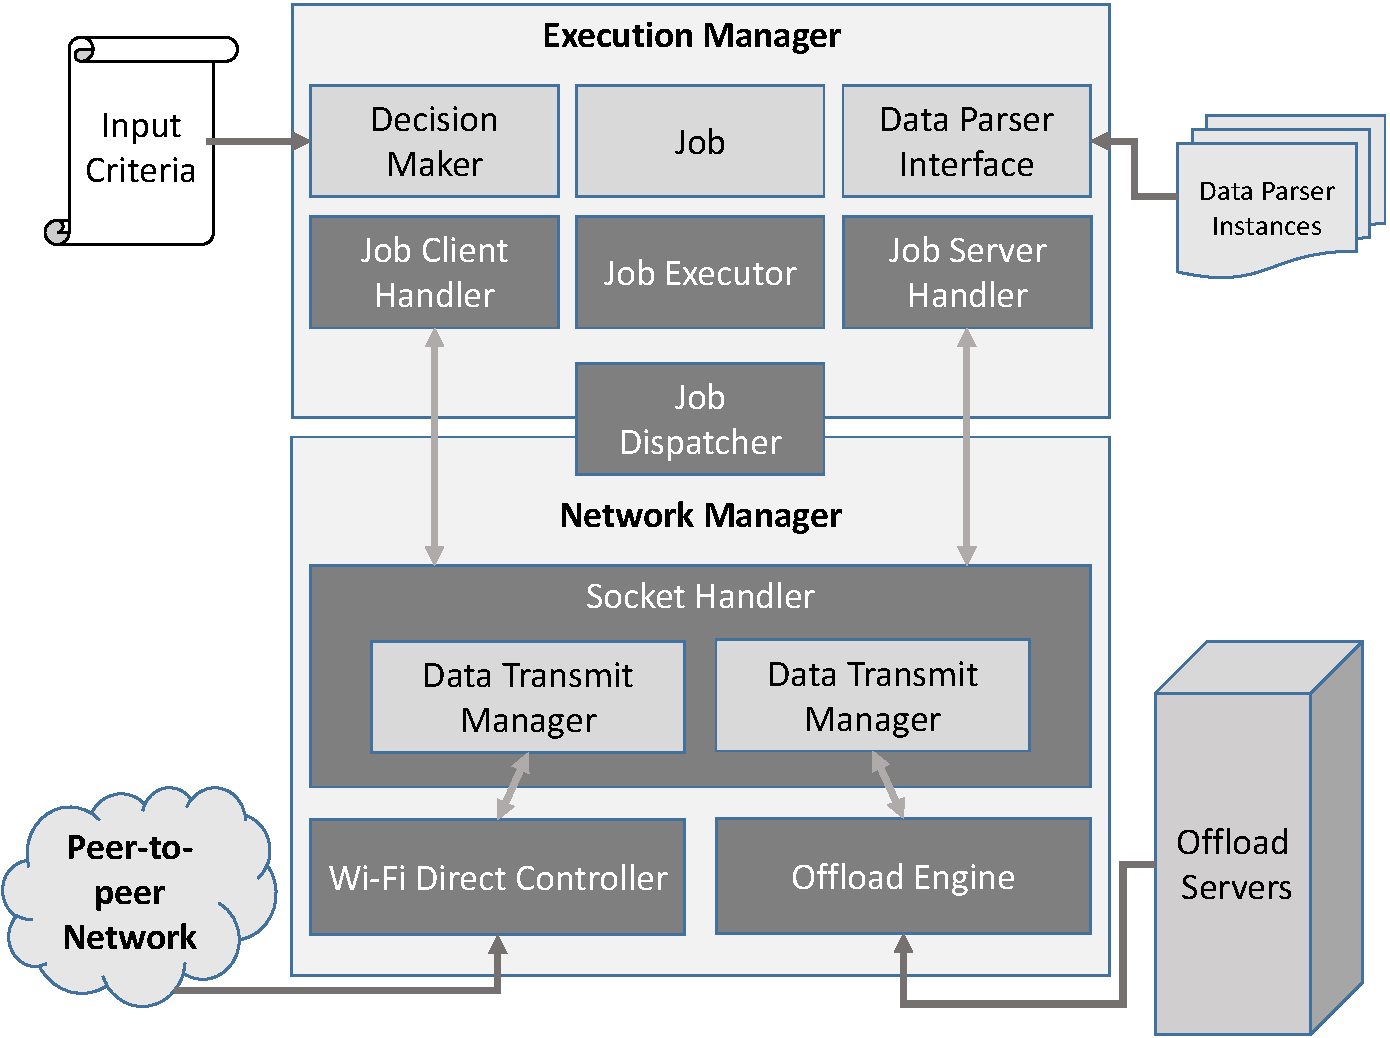
\includegraphics{data/jobShareArch.pdf}
	}
	\caption{System architecture}
	\label{fig:architecture}
\end{figure}


\subsection{Approach Overview}
%need a general description
%need to edit more
To achieve our goals---easy usage BLAH BLAH, , our system design choice is hiding the complexity of implementation details and open to the developers the capability of customization. Figure \ref{fig:architecture} describes the internal architecture of a typical application using our programming model. Our system comprises of two main components: (1) \emph{Wi-Fi Network Manager} (\emph{WNM}) manages connections between device to device, device to offload server, data transmission via sockets, connection discovery and establishment. For application programmers, the \texttt{WiFiNetworkManager} interface provides a simple API interface to easily form a closed range distributed network; (2) \emph{Execution Handler} provides abstract functionality for job definition, execution and distribution. Equipped with \texttt{DecisionMaker} sub module, \texttt{Execution Handler} can distribute jobs with appropriate amount data to the corresponding device to bring the highest optimization in terms of performance and energy consumption. In the next following sub sections, we will discuss into the details of the system architecture.

\subsubsection{WiFi Network Manager}
To establish connections between nearby mobile devices over the WiFi network, we utilized the WiFi Direct technology, the new feature available from Android APIs 4.0. In particular, \texttt{WiFiDirectController} of \texttt{WNM} hides the complexity of Wi-Fi Direct implementation. Holding an instance of \texttt{WifiP2pManager}, \texttt{WiFiDirectController} discovers available peers, establishes connections, and keeps track of the connections. As aforementioned in the previous section, to leverage computational offloading when a WiFi access point (AP) is available, the \texttt{OffloadEngine} module initiates a connection with our cloud-based offloading server \cite{kwon+:mobilesoft2015}, thus executing the job at a powerful remote server instead of looking for nearby devices. By providing transparent operations between the offload server and nearby mobile devices, our approach separates a job implementation from distributed execution models.

When an application starts, \texttt{WNM} calls \texttt{discoverPeers()} to search for available offloading servers registered in its configuration file, as well as spread acknowledgments to inform its availability to the other peers. If any offloading server or nearby devices receive discovery message, its \texttt{WNM} module updates the new caller to its available device list, then simultaneously sends their information back to the caller in a JSON object \ref{ss_dfp}, the same reactions will occur with the other peers. When all the devices are updated with the available device list, the network is organized as described in Figure \ref{fig:forming}.

\begin{figure}
	\centering
	\resizebox{0.5\textwidth}{!}{
		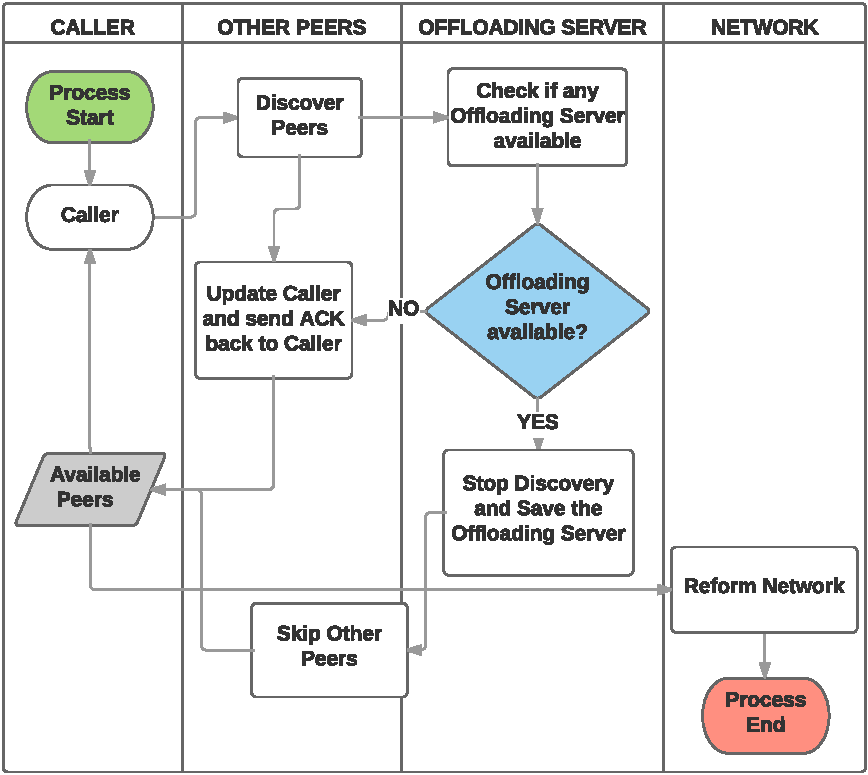
\includegraphics{data/discoverPeers.pdf}
	}
	\caption{Establishing a network connection between devices}
	\label{fig:forming}
\end{figure}


Once each mobile device receives all the required information from other mobile devices, they can be connected. We provide the method \texttt{connectToADevice()} holding \texttt{WiFiDeviceInfo} as one input parameter to invoke the handshake with another device. Once connection established, the device actively invoked will be assigned as client, which utilizes the \texttt{ClientSocketHandler} to listen to a client socket. The device passively received the invocation will be promoted as server and use the \texttt{ServerSocketHandler} to initiate server socket with an random port. If the invoked device is already a server, it will maintain its current state and continuously accept the new client. Moreover, since a device can either be a server to some peers, or serve as client to the others, this method is able to build up a close range peer-to-peer network.

Both \texttt{ClientSocketHandler} and \texttt{ServerSocket Handler} are constituted by a sub module named \texttt{Data TransmitManager}, which periodically observes input and output streams of parent socket (Can be either server or client socket) to verify checksum, check data consistency, send/receive data from the socket. Inheriting the \texttt{TransmitManager} abstract class, developer can instantiate their own version of \texttt{DataTransmitManager} to customize the data consistency checker or improve security. 

\subsubsection{Execution Handler}
\emph{Execution Handler} handles job definition, execution and distribution, where \texttt{Job} (See \ref{prog_model}) is executable unit defined by developer at runtime. By analyzing information of other mobile device list, \texttt{DecisionMaker} module will select a number of highest responsibile devices and decide jobs with appropriate amount of conjunctional data, then by \texttt{JobDispatcher}, dispatch them using to those devices. On each remote device or offload server, \texttt{Job} and its partial data will be deserialized and executed by \texttt{JobExecutor} in synchronous mode. After that, the results will be return back to the caller by \texttt{JobClientHandler} and \text{JobServerHandler}. To facilitate adaptation with data heterogeneity, we define \texttt{DataParser} as a loosely coupled interface of \texttt{Job} to support determining mechanisms for: (1) serialization/deserialization object into binary format which is compatible for TCP transmission, (2) task partitioning, and (3) placeholder initialization and concatenation. To make the data type comprehensive to system in terms of reading, parsing or memory allocating, developer needs to supply instructions by instantiating an implementation of Data Parser for that type. 

\subsection{Programming Model} \label{prog_model}
Our system has a simple programming model that enables the programmer can easily write remote functionality. Firstly, as described in code snippet (\ref{code:job_def}), we provide \texttt{Job} abstract class that should be extended by the programmer to specify which functionality should be executed remotely.

To support dynamic class loading in Dalvik VM, we provide the \texttt{DexCreator} commandline tool that compiles the \texttt{Job} Java file into a Dex package. The Dex package and sliced resources are packed as a \texttt{JobData} object by \texttt{JobDispatcher} and then dispatched to the available peers. Once a peer receives a \texttt{JobData} object, it first checks the checksum field to confirm the consistency, and then deserializes the object into \texttt{Job} and resources for the execution.

\begin{figure}
\noindent \shadowbox{%
\begin{minipage}{246pt}
	\begin{lstlisting}
	public abstract class Job {
	  public abstract Object exec(Object param); }
	\end{lstlisting}	
\end{minipage}}	
\noindent \shadowbox{%
\begin{minipage}{242pt}
  \begin{lstlisting}
public interface DataParser {  
  public Class getDataClass();
  public byte[] parseObjectToBytes(dataObject);
  public Object parseBytesToObject(byteArray);
  public Object getSinglePart(..., 
		numOfParts, sOffset, eOffset);    
  public Object createPlaceholder(jsonMetadata);
  public Object copyPartToPlaceholder(... 
					partDataObject, sOffset, eOffset);
  public void destroy(dataObject);  }
  \end{lstlisting}	
\end{minipage}
}	
\captionof{lstlisting}{Provided APIs (top: Job, bottom: DataParser)}
\label{code:job_def}
\end{figure}


\subsubsection{Data Parser}
The code snippet in Listing \ref{code:job_def} shows the main functionality of the \texttt{DataParser} interface that user needs to implement. The \texttt{DataParser} interfaces have the following abstract methods:
\begin{itemize}
	\item \texttt{getDataClass()} return data type.
	\item \texttt{parseObjectToBytes(object)} instructs system to serialize an object to binary array. In Android, not every object can be serialized, for instance Bitmap.  
	\item \texttt{parseBytesToObject(byte[])} deserialize a binary array back to object.
	\item \texttt{getSinglePart()} return a data slide bases on number of parts (\texttt{numOfParts}) and its \texttt{index}. Code snippet (\ref{code:get_single_part}) shows an example getting one slice from a bitmap by \texttt{index}. When app runs, \texttt{JobDispatcher} will use this method to partition the task into slices.
	\item \texttt{copyPartToPlaceholder()} Once partial result is retrieved from a distant peer, this function will instruct application to merge it to the placeholder.
\end{itemize}

In our initial prototype implementation, we provide three default parsers for bitmap images, texts, and GPS, respectively. 

\subsection{Runtime System} \label{scheduling}
Once a peer-to-peer network is constructed by our system, each peer participating in the network can distribute jobs to other peers. Specifically, before making a remote job execution, \texttt{DecisionMaker} determines available peers in accordance with the level of available resources by inquiring peers' status via a (\texttt{IRS}) message. Once one receives the IRS request, its \texttt{DecisionMaker} immediately responds to the request with the capability information of CPU, memory and battery usage at that time depicted in Figure \ref{fig:forming}.

%\begin{figure}
%\centerline {
%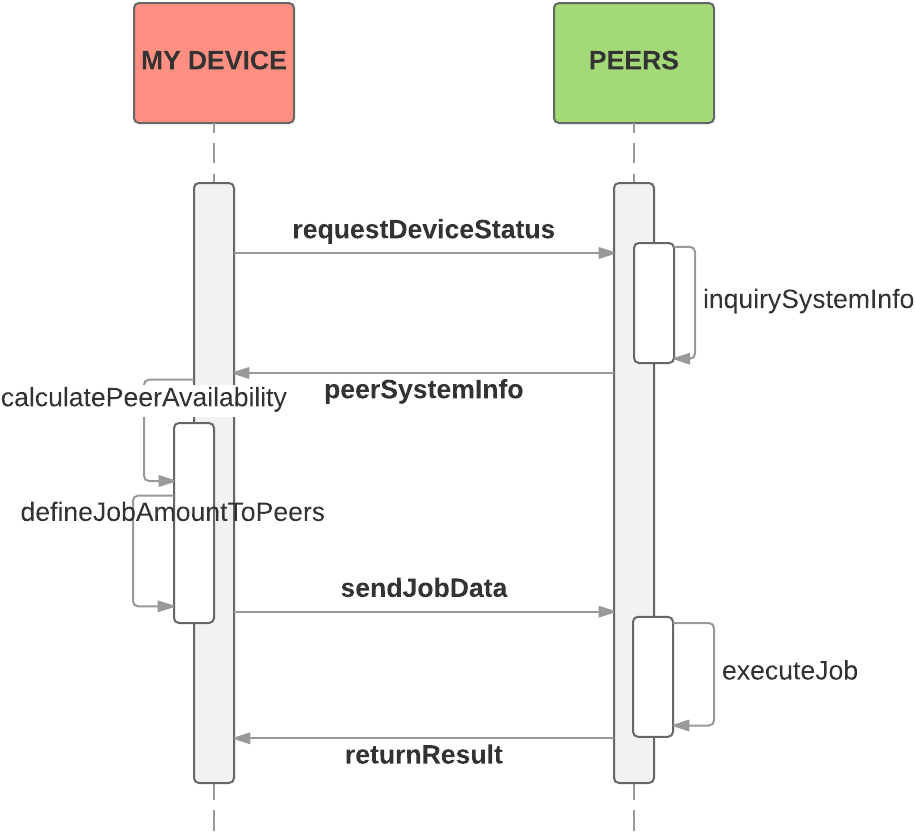
\includegraphics[width=0.45\textwidth, natwidth=915, natheight=837]{data/checkStatusFlow}
%}
%\caption{Workflow between mobile devices.}
%\label{fig:checkStatus}
%\end{figure}

\subsubsection{Finding available devices}\label{ss_dfp}

A mobile device at any time maintains a certain number of connection with the others. Before delivering jobs, it dispatches IRS messages to all the peers for acknowledgment of their availability ($RL$ - Level of Responsibility). If a peer receives an IRS, its \texttt{DecisionMaker} will capture its configuration and corresponding usage states to generate a response in JSON format, The code snippet (\ref{code:jsonResponse}) shows such a typical response.\\

\begin{figure}
\noindent \shadowbox{
\begin{minipage}{240pt}
\begin{lstlisting}
JSON : DeviceInfo {
  "device": "LG-Volt", "RL": 24.83,
  "availability": "off", "network": "low", "gps": "on",	
  "cpu": {"usage": "0.3", "speed": "1.3", "cores": 4},
  "memory": {"usage": "0.5", "total": 2},
  "battery": {"usage": 0.85, "total": 2800}}
\end{lstlisting}			
\end{minipage}}	\\
\noindent \shadowbox{%
\begin{minipage}{243pt}	
\begin{lstlisting}
JSON : Condition {"RL": "max", "gps": "on"}
\end{lstlisting}\end{minipage}}	

\captionof{lstlisting}{A JSON response format and initiative condition.}
\label{code:jsonResponse}

\end{figure}

Where \texttt{device} can be either device name (if it is device) or \texttt{server} (if it is offloading server), $RL$ is device's Level of Responsibility (for estimation of $RL$ and the other parameters, see \ref{ss_jqfp}), \texttt{availability} indicates whether device is feasible for handling job. \texttt{network} gives the network status, which can be either \texttt{high}, \texttt{low} or \texttt{off} (no connections), \texttt{gps} is information of GPS \texttt{on} or \texttt{off}. Finally \texttt{cpu}, \texttt{memory} and \texttt{battery} are statuses of the essential resources at the time of response. 

In any IRS response, \texttt{availability} is determined by the remote device which value can be assigned by \texttt{on} or \texttt{off}. The \texttt{off} value informs the caller that it is not available due to temporary lacking of resource, therefore eliminates the caller from sending jobs. Only the devices with \texttt{availability} is \texttt{on} will accept jobs for the execution. The value is given bases on whether device has bypassed the threshold of battery usage which is set by default at 0.8 (or 80\% overall usage). User can override those thresholds by updating the \texttt{availability-thresholds} in the configuration file before app initialization. 

In the above example (Code snippet \ref{code:jsonResponse}), the battery usage was 0.85 or 15\% remained, so the \texttt{DecisionMaker} on it stated that its \texttt{availability} is \texttt{off}, it won't be able to handle any jobs.

To make the system adjustable to wide range of resource usages with regard to energy and performance efficiency, the IRS criteria (Example in \ref{code:jsonResponse}) is added to the app configuration so that \texttt{DecisionMaker} can check by going through 3 below steps
\begin{itemize}
	\item \emph{If $RL$ is max}: Select one device having max $RL$ and match the other criteria, then finish.
	\item \emph{If offloading server available}: Select the first available server, then finish.
	\item \emph{If other criteria are matched}: Select a list of available devices having matched conditions.
\end{itemize}
The algorithm \ref{alg:select_peers} describes detailed the three above steps.

\begin{algorithm}

\caption{Selecting available peers}
\label{alg:select_peers}
\begin{algorithmic}[1] 
\begin{scriptsize}
\Function{selectPeers()}{}
\State Send IRS requests to all peers 
\State $CriteriaList \leftarrow IRSCriteria$
\State $P_{AV} \leftarrow HashMap(DeviceId, P)$

\If {$CriteriaList.RL = max$}
  \ForAll{$Resp_{IRS}$ in \{Incoming IRS Responses\}}
  	\State Find max $RL$ with other criteria in $CriteriaList$
  	\State \Return $P_{AV}$
  \EndFor
\EndIf

\ForAll{$Resp_{IRS}$ in \{Incoming IRS Responses\}}
  \If {$Resp_{IRS}[device] = server$}
  	\State Reset $P_{AV}$ 
  	\State $P_{Info} \leftarrow WiFiDeviceInfo[DeviceId]$
  	\State $P_{AV}[DeviceId] \leftarrow P_{Info}$
  	\State \Return $P_{AV}$
  \EndIf

  \If {All condition statements are satisfied} 
  	\State $P_{Info} \leftarrow WiFiDeviceInfo[DeviceId] + Resp_{IRS}[RL]$
  	\State $P_{AV}[DeviceId] \leftarrow P_{Info}$
  \EndIf
\EndFor

\State \Return $P_{AV}$
\EndFunction
\end{scriptsize}
\end{algorithmic}

\end{algorithm}

The algorithm \ref{alg:select_peers} explains how the caller select the suitable peers from its connection list. Where $P_{AV}$ stands for map of available peers and $P2pDevice$ is the device information list.\\

\subsubsection{Job quantitation for peers}\label{ss_jqfp}

The calling peer quantitates the jobs from a task to distribute to the other available devices in the network suitably. To achieve this, the $RL$ parameter will be used as the main coefficient for the split. 
 
To calculate $RL$ as well as the other parameters in IRS, retrieved from \texttt{/proc/stat} system file \cite{stat_explain}, the percentage of CPU usage is expressed by this following expression in two short consecutive times

\begin{equation}
\label{eq:cpu_usage}
Usage_{CPU} = \frac{(\sum{T_{CPU2}} - T_{Idle2}) - (\sum{T_{CPU1}} - T_{Idle1})}{(\sum{T_{CPU2}} - \sum{T_{CPU1}})}
\end{equation}

Where $\sum{T_{CPU}}$ is total time of running CPU and $T_{Idle}$ is idle time correspondingly in hertz. In term of memory usage, the $Usage_{Mem}$ can be determined by using \texttt{MemoryInfo} from Android API to retrieve $Mem_{Avail}$ and $Mem_{Total}$, so the $Usage_{Battery}$.

Since in the mobile device, the lower resource usage state states the higher availability, and the higher specifications represents the better responsibility. Then the level of responsibility of device can be simply summarized by the below expression

\begin{equation}
\label{eq:res_level}
%\begin{\footnotesize}
RL = \frac{N_{Cores} \times CPU_{Speed}}{Usage_{CPU}} + \frac{Mem_{Spec}}{Usage_{Mem}} + \frac{Battery_{Spec}}{Usage_{Battery \times 1000}}
%\end{\footnotesize}
\end{equation}

Where $N_{Cores}$ is number of CPU cores and $CPU_{Speed}$ is speed of single core in GHz unit, $Mem_{Spec}$ has GB unit and $Battery_{Spec}$ has uAh unit. At a certain time of that device, if $Usage_{CPU}$ is 0.3, $Usage_{Mem}$ is 0.5 (half of 1GB memory consumed), $Usage_{Battery}$ is 0.7 or 70\% used over a 2800uAh capacity battery, the value of $RL$ will be
$$RL = \frac{5.2}{0.3} + \frac{1}{0.5} + \frac{2800}{0.7 \times 1000} = 23.33$$

To reduce the latency and to avoid miscalculation at the calling peer, $RL$ is prematurely calculated by each available called peer and wrapped up in the IRS response sending back to the caller. 

In a P2P network comprising of $n$ devices, where $i$-device has responsibility level $RL_{i}$, the \texttt{DecisionMaker} will assign the job with carrying amount of data ($M_{i}$) which is equivalent to

\begin{equation} 
\label{eq:data_amount}
M_{i} = M\frac{RL_{i}}{\sum_{j = \overline{1,n}}{RL_{j}}}
\end{equation}

Where $M$ is total size of data in bytes. This below algorithm \ref{alg:assign_job} will represent the procedure that \texttt{DecisionMaker} judge the peer capability to assign the appropriate job. Where $M_{i}$ is quantity of job in binary length, $firstOffset$ and $lastOffset$ indicate the location of the data trunk in the whole.

\begin{algorithm}
\caption{Assigning a job}
\label{alg:assign_job}
\begin{algorithmic}[1]
\begin{scriptsize}
\Function{assignJobs()}{}
\State $M \leftarrow {getDataSize()}$
\State $RL_{Total} \leftarrow 0$ 
\For {$P$ in \{$P_{AV}$\}}
  \State $RL_{Total} \leftarrow RL_{Total} + P[RL]$
\EndFor
\\
\State $firstOffset, lastOffset \leftarrow 0$
\State $jobData \leftarrow Null$
\State $job \leftarrow {readJobFile()}$
\State $M_{C} \leftarrow 0$
\\
\For {$i = 1$ to $P_{AV}.length$}\\
  \State $M_{i} \leftarrow M\frac{RL_{i}}{RL_{Total}}$\\
  \State $firstOffset \leftarrow M_{C} $
  \State $lastOffset \leftarrow M_{C} + M_{i}$
  \State $jobData \leftarrow DataParser.getSinglePart($
  \State 
		\hspace{\algorithmicindent}
		\hspace{\algorithmicindent}
		\hspace{\algorithmicindent}
		\hspace{\algorithmicindent}
		\hspace{\algorithmicindent}
						$firstOffset, lastOffset)$
  \State $dispatchJob(\{job, jobData\})$\\
  \State $M_{C} \leftarrow lastOffset$
  
\EndFor

\EndFunction
\end{scriptsize}
\end{algorithmic}
\end{algorithm}

\subsection{Estimating Energy Consumption in WiFi Environment}
Assume that we have a Wi-Fi peer-to-peer network available with $n$ devices, each device at a certain time has level of responsibility $RL_{i} (i = \overline{1,n})$. According to the section \ref{scheduling}, if $E$ is the energy consumed by the application for only completing the task regardless of other ambiances, the total energy $E_{0}$ will be

$$E_{0} = E + E_{w}$$

Where $E_{w}$ is energy the app requires for waiting. Also, 

$$E_{p2p} = E(\frac{RL_{0}}{\sum_{i = 1}^{n}{RL_{i}}}) + E_{WiFi} + E_{w}$$ 

Where $E_{WiFi}$ is energy consumed by Wi-Fi for sending jobs to other peers.

In this estimation we skipped considering $E_{w}$ since it will depend on appearance of applications. If application have no GUI like system background services, $E_{w}$ will cause very little effect. From the two above equations, we can get the difference energy consumption between the two job processing mechanisms $E_{Diff}$ 

$$E_{Diff} = E_{0} - E_{p2p}$$ 

or 

\begin{equation}
\label{eq:energy_diff}
E_{Diff} = E(1 - \frac{RL_{0}}{\sum_{i=1}^{n}{RL_{i}}}) - E_{WiFi}
\end{equation}

According to \cite{wifi_energy}, Wi-Fi caused battery drained linearly by time during the transmission, particularly the drain can be represented by $y = 17.01x - 0.93$ for downloading and $y = 17.31x - 2.28$ for uploading, where $y$ stands for percentage of battery consumed when using Wi-Fi for a period of $x$ hours. Therefore, under non-adventitious circumstances, equation (\ref{eq:energy_diff}) infers that in a mobile system with a certain number of devices in different levels of responsibility, if E is big enough, or in the other words, if the task to perform is big enough, then $E_{Diff} > 0$ will happen, thus deploying a peer-to-peer cluster will give the great benefit in term of energy efficiency. The bigger value of $E_{Diff}$, the more benefit we will archive.

\subsection{API Usage Scenario}

The library should be simple, so that developer can integrate within just a few steps. This section will describe step-by-step the way to utilize our API to enable a typical peer-to-peer network.

\subsubsection{Defining a Job}

Job implementation is the prerequisite work to determine what to execute on the remote device and how to cast and manipulate data from the abstract object. According to section \ref{job-description}, developer needs to implement the Job class file separately by overriding the \texttt{exec()} method and cast the input abstract parameter to the concrete. Then run the \texttt{DexCreator} tool on the Job class to compile and compact it into the DEX jar package. The final outcome is the \texttt{job.jar} file, it should be saved in the internal storage of the caller device. To simplify, we can store it in the \texttt{Download} folder.  

\subsubsection{Implementing an Application Using APIs}

This sub section will describe 3 basic steps to implement an Android application to utilize our APIs

\paragraph{Message Handler}

The Message Handler is required to instantiate at the beginning. In particular, an instance of \texttt{UIHandler} is initiated to receive messages from system when it goes into runtime. While system is in progress, the log and information messages will periodically be returned with label \texttt{MAIN\_INFO} (Code snippet \ref{ui_handler}). When each job result comes, \texttt{JobHandler} will collect and handle by  to partially put into a placeholder. When all results arrived, the placeholder with label \texttt{MAIN\_JOB\_DONE} will be returned to inform the completion of job collaboration, as well as bring the final result back to the main app UI.\\

\begin{figure}
\noindent \shadowbox{%
\begin{minipage}{239pt}	
	\begin{lstlisting}
Handler mainUiHandler = new Handler() {
	public void handleMessage(Message msg) {
		switch (msg.what) {
			case Utils.MAIN_JOB_DONE: { ... }
			case Utils.MAIN_INFO: { ... } }	} };
	\end{lstlisting}
\end{minipage}
}
\captionof{lstlisting}{UI handler}
\label{ui_handler}
\end{figure}

\paragraph{Data Parser}

Secondly, developer needs to declare \texttt{DataParser} to determine data-type and parser to equip for manipulating data at run-time (see sub section \ref{job-description}). \texttt{JobHandler} is the main component which wraps up the complexity , and exposes only the necessary functions like \texttt{discoverPeers()} and \texttt{dispatchJob()}. To send ACK messages to other peers for exchanging acknowledgments and reforming network, we need to call \texttt{discoverPeers()} function on the program, this work should be done as soon as application starts.\\

\begin{figure}
\noindent \shadowbox{%
\begin{minipage}{245pt}
  \begin{lstlisting}
public Object getSinglePart(object, sOffset, eOffset) {
  Bitmap bmpData = (Bitmap) data;
  int pWidth = eOffset - sOffset;
  return Bitmap.createBitmap(bmpData, sOffset, 
									0, pWidth, bmpData.getHeight()); }
  \end{lstlisting}	
\end{minipage}}	
  \captionof{lstlisting}{Example of \texttt{getSinglePart()} for Bitmap}
  \label{code:get_single_part}

\end{figure}

\paragraph{Discovery Peer and Dispatching Jobs}

When network is formed and connections are held from some of the peers, \texttt{dispatchJob()} will be call to locate the resources and job which predefined in local storage, it then invokes \texttt{DecisionMaker} (sub section \ref{scheduling}) for job splitting and binary serialization. Finally jobs will be dispatched over the socket\\

\begin{figure}
\noindent \shadowbox{%
\begin{minipage}{245pt}
	\begin{lstlisting}
dataParser = new BitmapJobDataParser();
jobHandler = new JobHandler(this, dataParser);

jobHandler.setSocketListener(
	new JobHandler.JobSocketListener() {
		@Override
		public void socketUpdated(... isConnected){
			...
		}});
deviceList.setAdapter(jobHandler.getDeviceListAdapter());
jobHandler.discoverPeers();

String dataPath = downloadPath + "/mars.jpg";
String jobPath = downloadPath + "/Job.jar";
jobHandler.dispatchJob(dataPath, jobPath);
\end{lstlisting}
\end{minipage}}

\captionof{lstlisting}{Using DataParser and JobHandler}
\end{figure}

\section{Evaluation}
\label{sec:eval}

\subsection{Micro Benchmark}
We started the evaluation with micro benchmarking energy consumption of the system when mobile devices maintain connections in idle state, to figure out the cost of network maintenance overhead. Using Moosoon Power Monitor device \cite{moosoon} to replace battery and measure on one caller, we evaluated overhead bases on cumulation of energy consumption by time. The Figure (\ref{fig:microb_24}) shows the outcome of the caller measuring from 0 to 100 seconds when preserving connections with 1, 2 and 3 other peers. 

\begin{figure}
	\hspace*{-0.15cm}
	\resizebox{0.5\textwidth}{!}{
		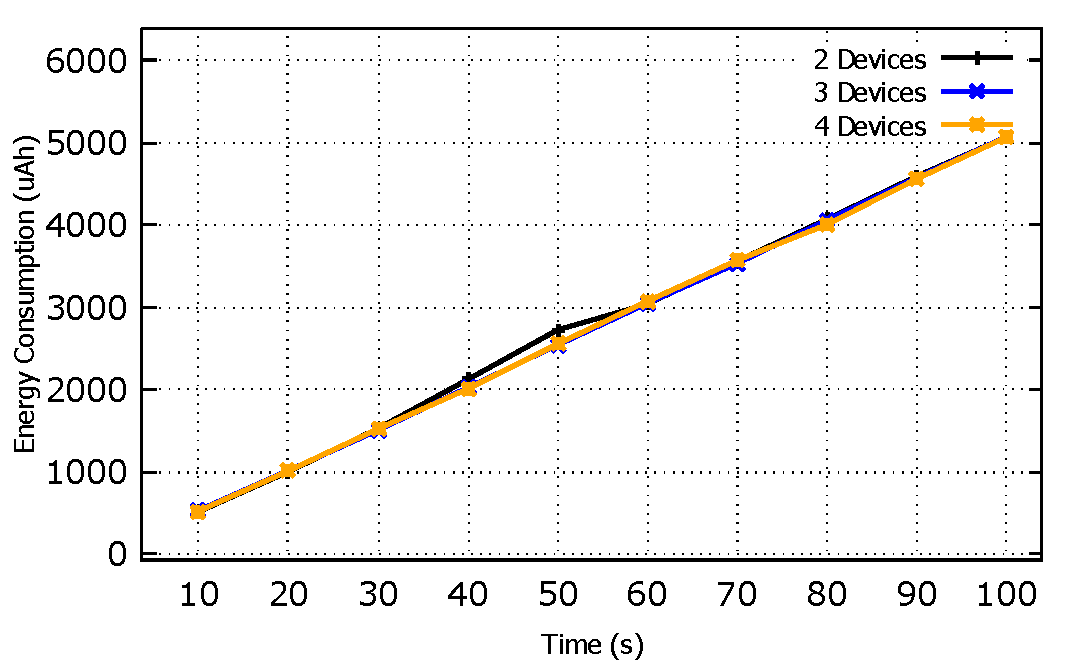
\includegraphics{data/ovh.pdf}
	}
	\caption{Energy consumption cumulation on caller in multiple clusters}
	\label{fig:microb_24}
\end{figure}

According to the figure \ref{fig:microb_24}, it is revealed that in idle condition without transmitting any data, the energy consuming variability on each device within the P2P network is linear and mostly identical at any time, regardless of number of devices to which it connects. This result is completely harmonized with results from \cite{wifi_energy}, especially since we transmit the same amount of data regularly over Wi-Fi connection. From the statistic information we collected, the energy variability of one device within P2P network in idle condition can be represented by the below linear formula

\begin{equation}
\label{eq:wifi_overload}
E_{WiFi} = t \times 50
\end{equation}

Where $t$ is accumulated time in milliseconds and $E_{WiFi}$ is energy used by system in uAh (micro ampere hour) unit.

\subsection{Case Study}
To measure the performance of the system equipped with our APIs, we decorated a small testbed with collaboration of 5 different Android devices to perform our 3 test cases:
\begin{itemize}
	\item \textbf{Image Processing} we will initiate the P2P network test to perform blurring a large scale image which is unable to process at any of our devices. Particularly, to process an image with size $4000 \times 4000$ and 4 bytes to express each pixel color, application must spare the amount of memory equivalent to 64MB which is way too much for a device, which occasionally returns out of memory exception.
	\item \textbf{Internet Remote Access} brings the Internet access capability to a device having no Internet connection or limited bandwidth by relying on other Internet-featured peers.
	\item \textbf{GPS Sharing} establishing a GPS connection is proof of high energy consuming. It would be impossible for a device with low battery to keep update with GPS frequently. We will base on N-DIST to build a simple system so that one device can benefit GPS locations from the healthier devices.
\end{itemize}

\subsection{Case Study Implementations}

\subsubsection{Image Processing}
We applied blur effect, one of the energy consuming process on images. We run the test repeatedly on two image inputs, the first image has size $2500 \times 1405$ and the second size is $4326 \times 2856$. For the second image, with 4 bytes allocated for each pixel, device must allocate around $50MB$ of heap to open and hold another $50MB$ for the result, thus leading to app crash all the time. The problem will only be solved by other collaborative peers to solve overload in terms of memory and energy consumption.

\paragraph{Design}
The most important part when applying APIs for image processing is defining the \texttt{BitmapDataParser} (see code snippet (\ref{code:job_def})) with a divide strategy in vertical cut. For an input image, the \texttt{firstOffset} and \texttt{lastOffset} will decide the first and last offsets of the vertical cut correspondingly throughout the width, from the top to the bottom edges. The algorithm of the vertical cut is described in the code snippet (\ref{code:get_single_part}). Regarding the placeholder, we override the \texttt{getJsonMetadata()} method to return a simple JSON string like below:

%\noindent \shadowbox{%
%\begin{minipage}{245pt}
	%\captionof{lstlisting}{JSON for initiating placeholder}
	\begin{lstlisting} 
	JSON { "width": 4326, "height": 2856 } 
	\end{lstlisting}
%\end{minipage}
%}

The method \texttt{createPlaceholder()} will parse this JSON object to obtain \texttt{width} and \texttt{height} as the inputs to initiate an empty placeholder bitmap. Finally \texttt{copyPartToPlaceholder()} method will place the partial result bitmap into its correct location on the placeholder defined by \texttt{sOffset} and \texttt{eOffset}.\\

\begin{figure}
\noindent \shadowbox{%
\begin{minipage}{245pt}
	\begin{lstlisting}
public Object copyPartToPlaceholder(placeholder, 
										part, sOffset, eOffset){
	Bitmap bmpPart = BitmapFactory.decodeByteArray(part...);
	int pieceWidth = partBmp.getWidth();
	Canvas canvas = new Canvas(placeholder);
	canvas.drawBitmap(bmpPart, sOffset, 0...);
	return null;
}
	\end{lstlisting}
\end{minipage}}
	\captionof{lstlisting}{Merging the result}
\end{figure}

When all the partial bitmaps received, system throws a message titled \texttt{MAIN\_JOB\_DONE} to the UI which \texttt{msg.obj} contains a final bitmap.

\begin{figure*}
	\centering
	%\resizebox{0.39\textwidth}{!}{
	%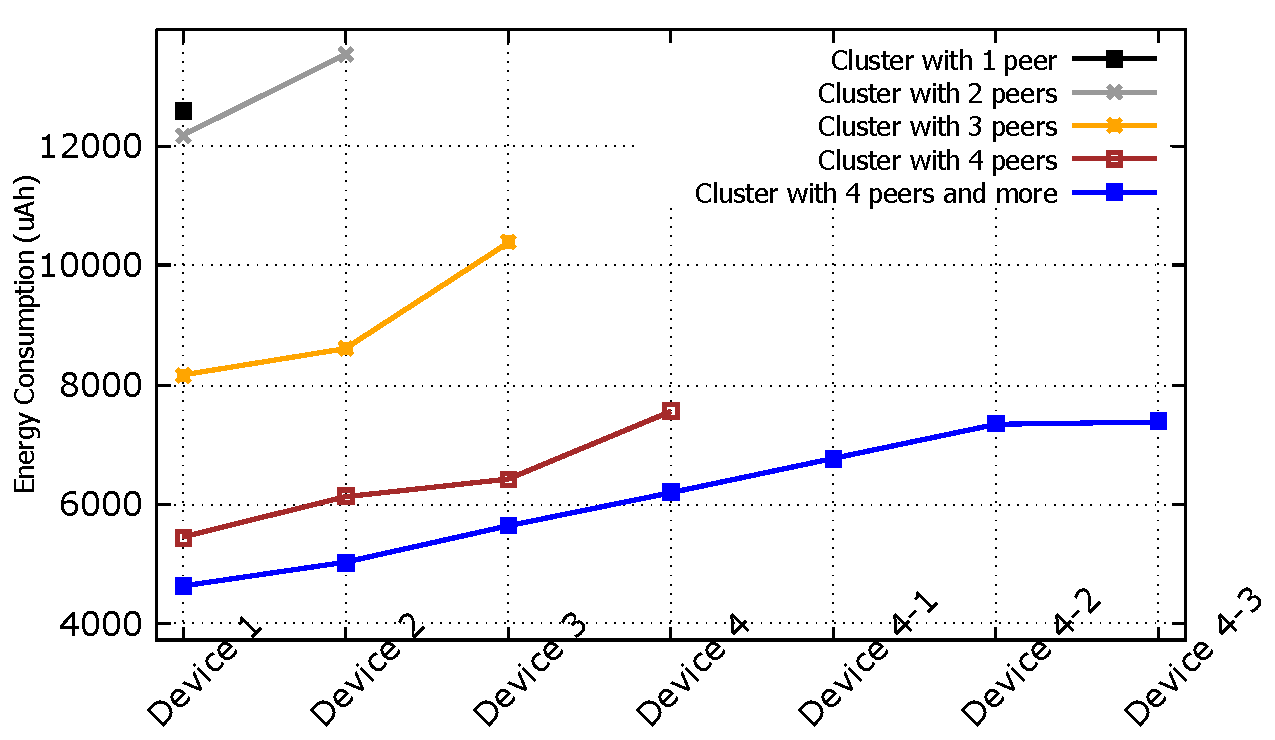
\includegraphics[width=0.32\textwidth]{data/img_large_perf_full.pdf}
		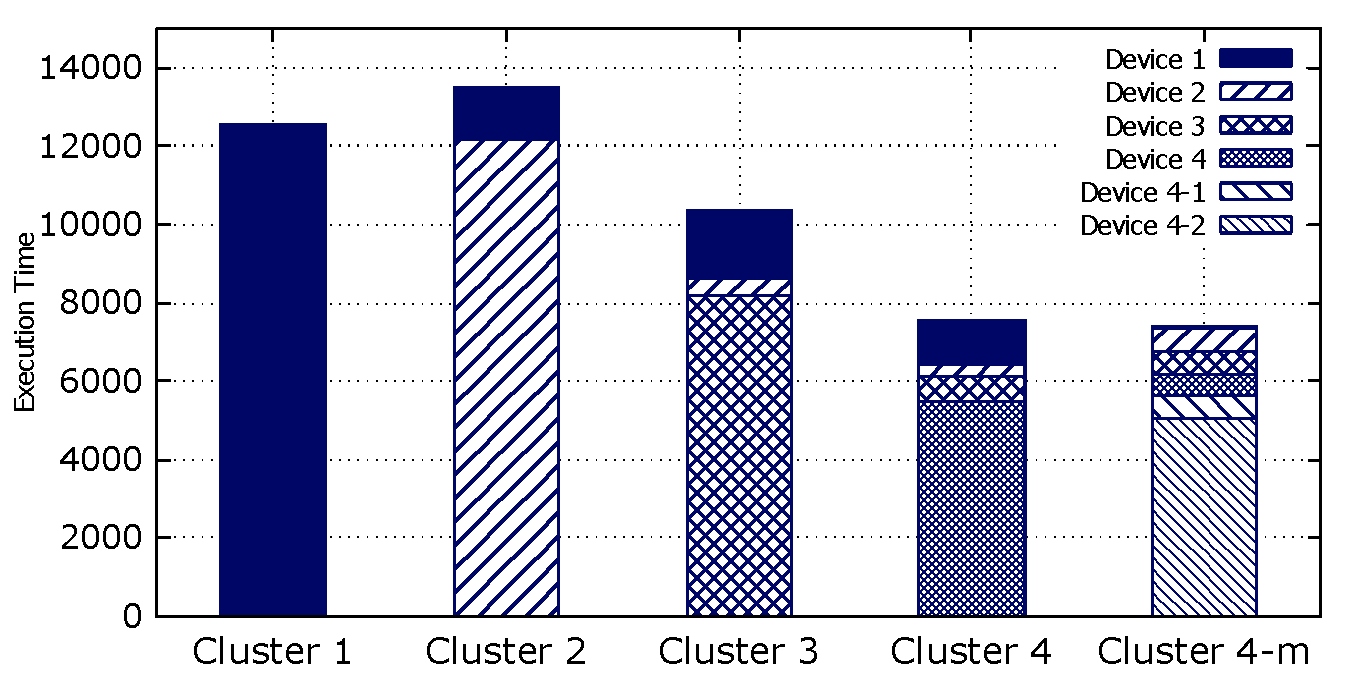
\includegraphics[width=0.39\textwidth]{data/img_perf.pdf}
		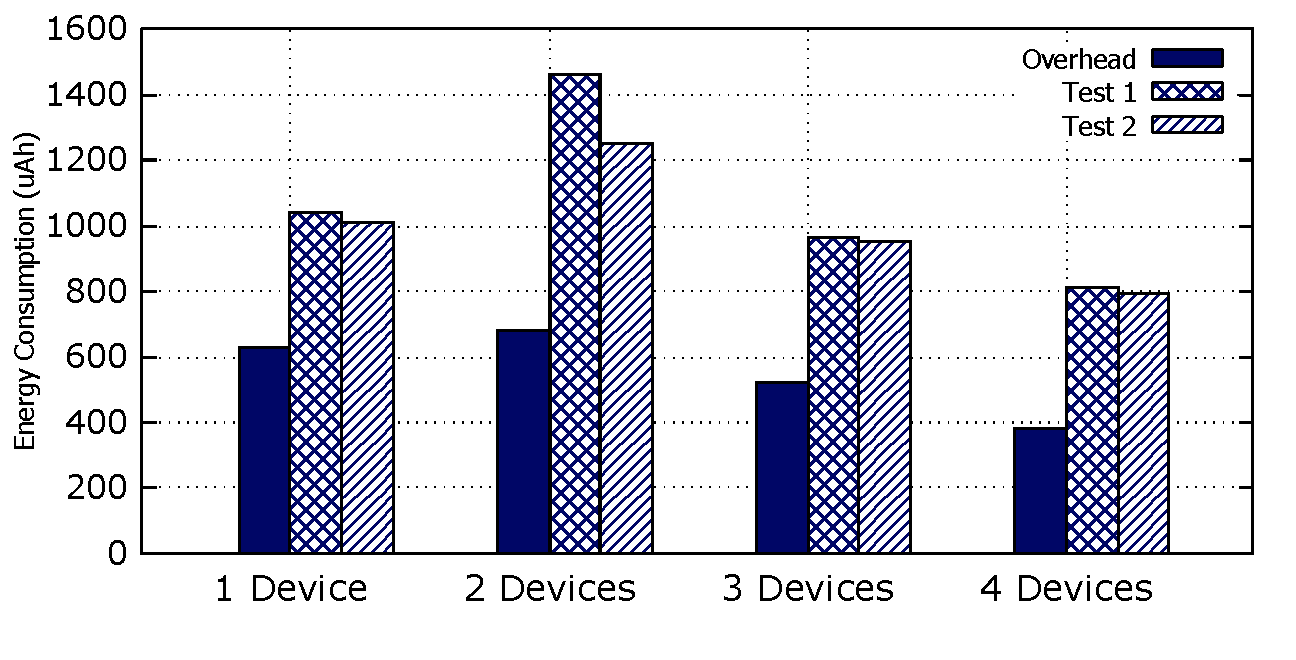
\includegraphics[width=0.45\textwidth]{data/img_energy.pdf}
	%}
	\caption{Performance and energy consumption of the large image processing tests in multiple clusters}
	\label{fig:cluster_performance}
\end{figure*}

\paragraph{Performance with large scale image}
Running the large scale image test case throughout 50 tests by increasing number of devices from 1 to 5 within the network, we found that the test case doesn't work if there is only one device standing desolately. By utilizing 2 threads for the image process on that single device, we realized that only 1 thread works, the another does not due to out of memory exception, and the processing time to complete half of the task is $12,581ms$. 

By increasing the number of devices in network from 2 to 5 and sharing the task by sending jobs to the other peers, we gathered average statistic data in 20 tests as in the Figure \ref{fig:cluster_234} (in cluster with 2, 3, 4 and more). In the Figure, the grey line shows that $12,187$ is the time in millisecond the caller received response from device \#1, and $1354ms$ later it received response from the second device. In other words, the caller accomplished the task within $13,541ms$. The same behaviors happened in the other lines, and it is seen the blue line which 4 more devices get involved will complete the task in the shortest time ($7387ms$), also each device finished its assigned job earlier in compare with them in the other clusters. 

The Figure \ref{fig:cluster_performance} summarized performance in terms of time consuming between multiple clusters. Noticed that system didn't fully work with only one device, and the one feasibly working thread in that single device took $12,581ms$ to complete, similar speed with 2-peer system. However speed is rapidly increased when more peers joined the network, especially with 4 devices, it is twice as fast as having 2 devices. Multiple threading is applied on the 4th device but did not sanitize very much the performance. 

To perform energy consumption on each cluster, we used Moosoon Power Monitor and measure the velocity of energy drained on a single mobile device when utilizing power from the other peers. Figure (\ref{fig:cluster_performance} - right) shows the energy measurement results from the two consecutive tests, although the two tests gave the big gap when executing 2 device cluster, in general the variability of energy consumption within multiple clusters matches with time consumption one. By running the two consecutive tests with the same input for 20 times, we realized that the results didn't change, and by utilizing 3 or more devices, we can significantly reduce the amount of energy required for the task, sometimes up to 25\%. However when we increased the number of devices in cluster, we didn't get the performance raised up at corresponding value linearly, this can be explained by Amdahl's law \cite{amdahl}. Throughout our experiments, the number of devices at 3 to 5 will give the maximum benefit in terms of energy saving and device usage productivity.

\paragraph{Performance with normal scale image}
To make any device in the network to be feasible for image processing, we reduced the input image size to $2500 \times 1405$. By reconfigure the cluster from 1 to 4 devices and measure total execution time on the callers, we gathered performance data between them like in the Figure \ref{fig:small_img_perf}. From our statistic data, the total time consumed by one device to run on itself is slightly fluctuated around $5400ms$ between multiple measurements, but if one more device join the network the time consuming is decreased to $3500ms$ which is 35\% faster. When more devices (3rd and 4th) participated, performance will continuously increase although their finishing time is largely varied. Especially 4 devices will collaboratively execute twice as fast as one device, or 50\% faster in all of our measurements.

\begin{figure*}
	\centering
	%\resizebox{0.45\textwidth}{!}{
		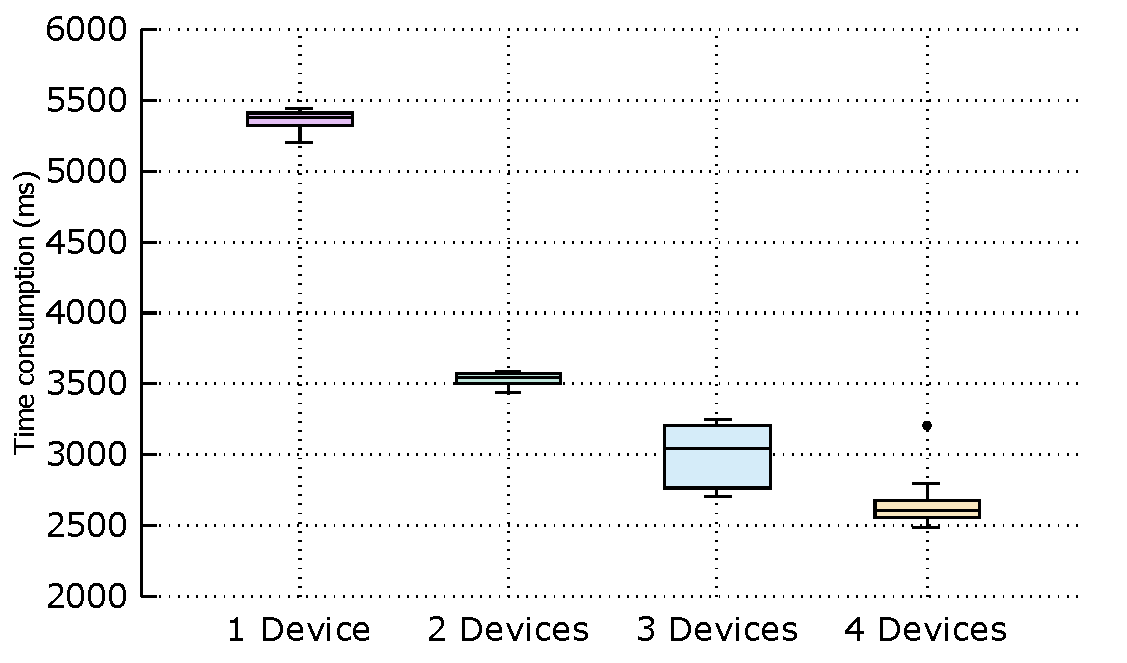
\includegraphics[width=0.48\textwidth]{data/img_small_perf_full.pdf}
		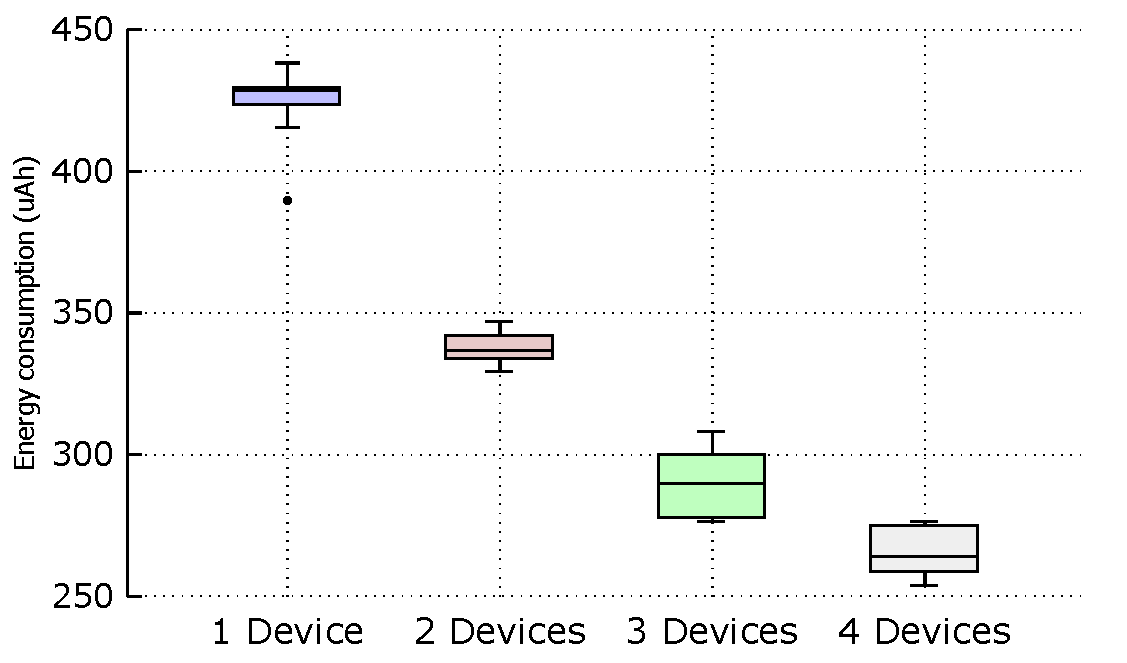
\includegraphics[width=0.45\textwidth]{data/img_small_energy.pdf}
	%}
	\caption{Performance and energy consumption from the image processing tests with normal size image in multiple clusters.}
	\label{fig:small_img_perf}
\end{figure*}

Basically the variability and fluctuation of energy consumption will reflect the performance, Figure (\ref{fig:small_img_perf} - right) displays the details. Through our experiments, running the cluster with 2 devices will preserve 20\% energy compare with 1 device, the number is better with 3 devices at $34\%$ and 4 devices at $37.5\%$ respectively.\\

%\begin{figure}
	%\centering
	%\resizebox{0.39\textwidth}{!}{
		%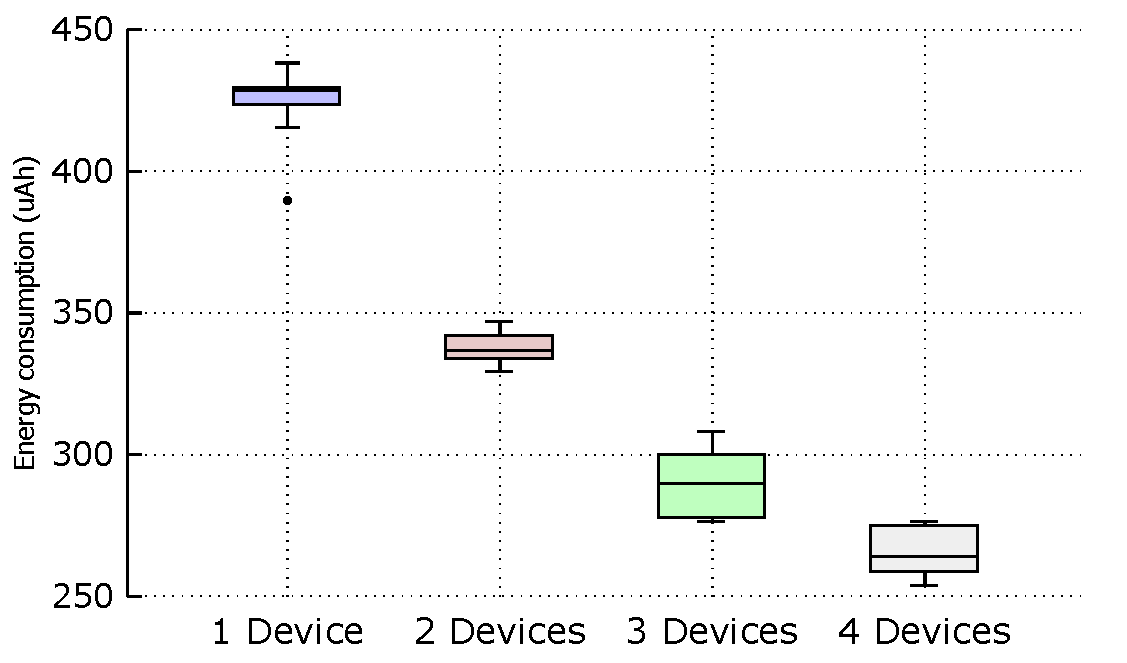
\includegraphics{data/img_small_energy.pdf}
	%}
	%\caption{Energy consumption from the image processing tests in multiple clusters.}
	%\label{fig:small_img_energy}
%\end{figure}

\subsubsection{Internet Remote Access} 
Theoretically, remote accessibility won't help reducing the amount of bytes downloading, but the speed is guaranteed to be ameliorative since the downloading process is scattered over a number of devices, therefore energy will be consumed less. 

\paragraph{Design}

To apply APIs for this application, from the caller we dispatch job requests, which contains information of job with resources are URL, number of parts and index, to the peers having \texttt{IRS[network]} at \texttt{high} or \texttt{low} (See ). At each peer, when request is received, it executes job to load URL to achieve page in HTML code. Then it will parse the HTML to detect resource links including multimedia resources (images, audio, videos), CSS, and JS. Depend on the number of parts and index, it narrows down the amount of resources and attempt downloading and put into a ZIP file before throw back to the caller.

According to our system architecture, the caller needs to prepare a placeholder to hold every incoming results. For this test case, the placeholder is designated as a sub folder in the \texttt{Download} folder. When result comes as a ZIP file, contents will be extracted and filled into the placeholder folder. The final HTML file will contain all the modified resource links which locate at the same folder. Finally, the local HTML file can be open by Android Web browser component using a local web server, for instance TinyHTTPd \cite{tinyhttpd}.

\paragraph{Performance}
Figure \ref{fig:net_clusters_perf} describes performance of multiple clusters from 1 to 4 peers and one peer has a few threads (for simulating high performance) when remotely rendering web pages from CNN URLs. The figure describes the execution time of each peer in each cluster after being assigned job, and the peak is reached when the last peer completed. In the cluster with only one device, that device works desolately without any peer contacts; it will download web pages from the internet by opening Wi-Fi connection. It is obvious that executing Internet Remote access brings the high benefit in terms of performance that rendering time reduced almost half when at least 3 peers participating network. 

\begin{figure*}
	\centering
	%\resizebox{0.45\textwidth}{!}{
		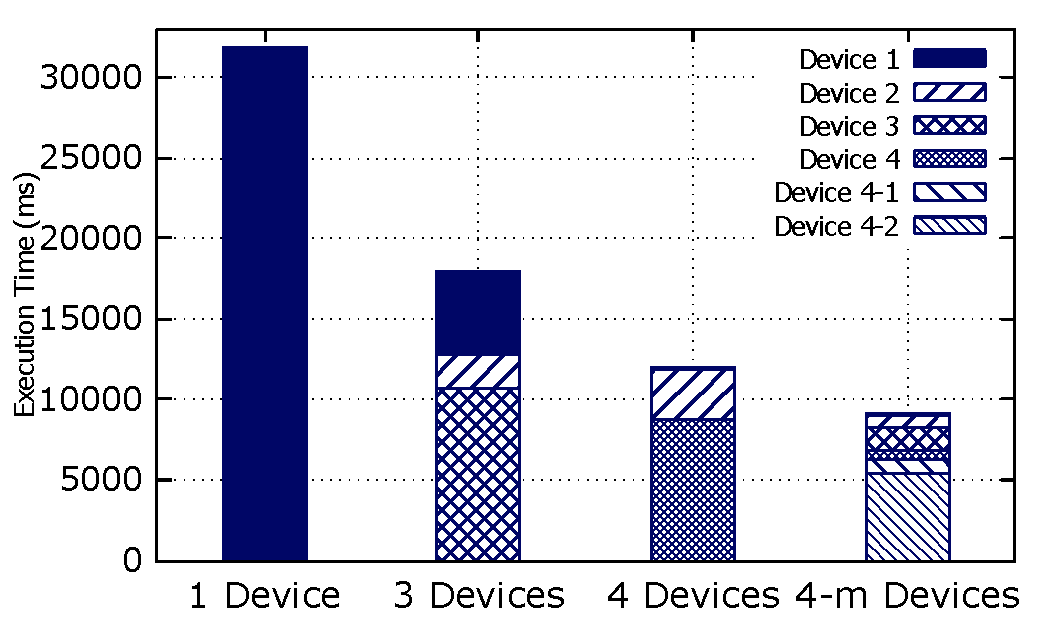
\includegraphics[width=.45\textwidth]{data/net_perf_01.pdf}
		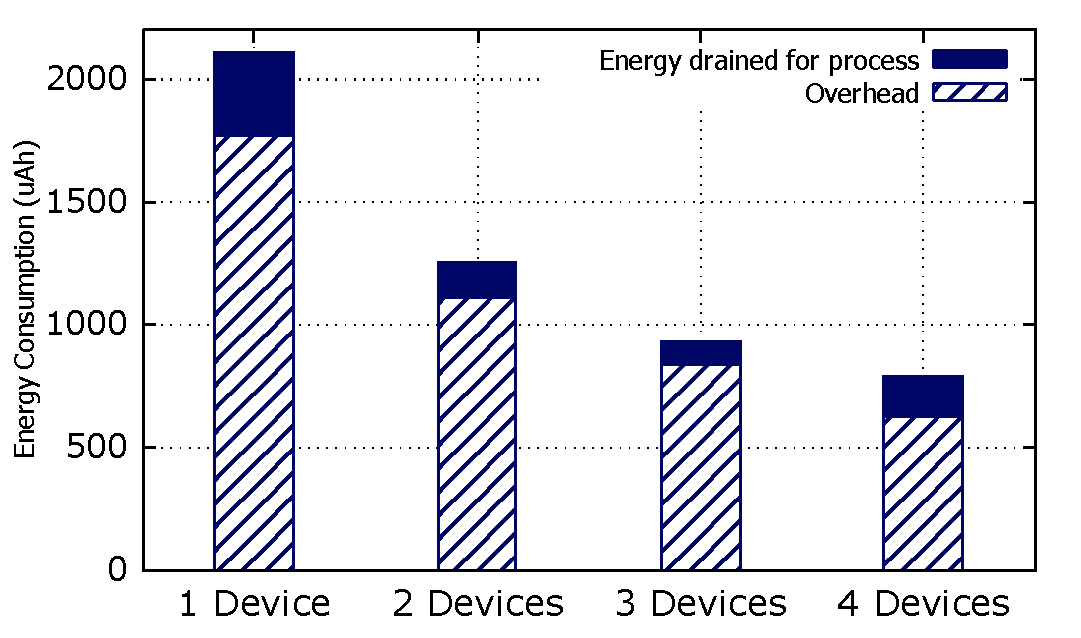
\includegraphics[width=.45\textwidth]{data/net_energy.pdf}
	%}
	\caption{Performance and energy consumption comparison for Internet sharing}
	\label{fig:net_clusters_perf}
\end{figure*}

To evaluate energy consumption, we performed the same tests like the first test case by measuring in multiple clusters with overheads and when remotely rendering web pages. From the outcome of energy test (Figure \ref{fig:net_cluster_energy}), we realized that by handing over computation utilizing system resources (Here is Internet accessibility) over peer-to-peer network with multiple peers will help reducing significantly energy consumed, particularly more than a half in compare with a solo device. The differences between the total energy and overheads are not fluctuated much between the multiple clusters, this can be easily explained by \cite{wifi_energy}.\\

%\begin{figure}
	%\centering
	%\resizebox{0.39\textwidth}{!}{
		%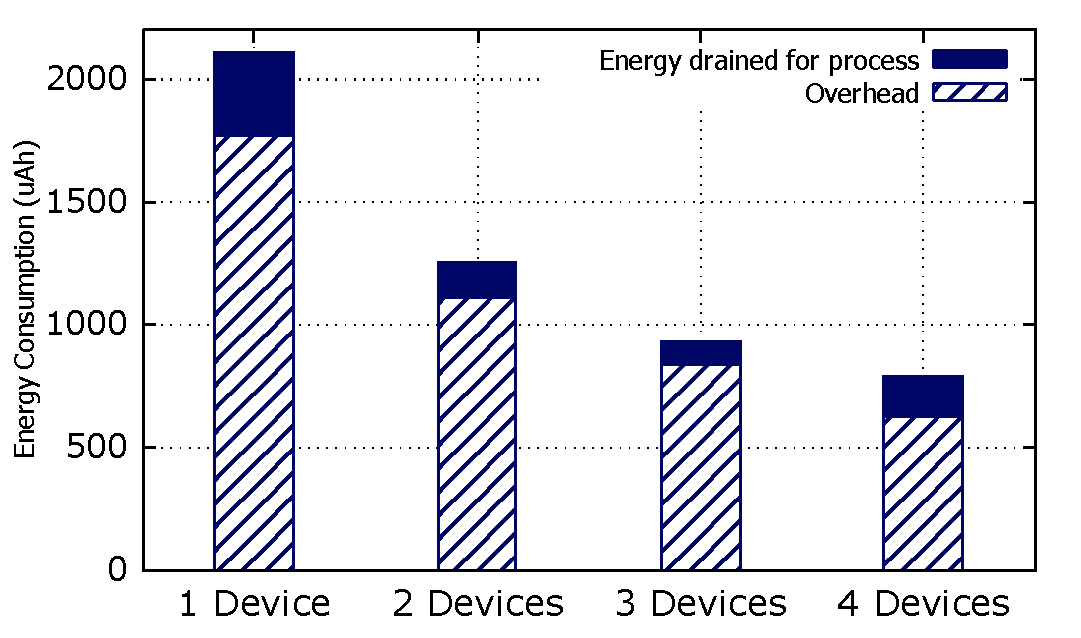
\includegraphics{data/net_energy.pdf}
	%}
	%\caption{Energy consumption of clusters for Internet sharing}
	%\label{fig:net_cluster_energy}
%\end{figure}

\subsubsection{GPS Share}
Connecting and retrieving GPS location is really energy consuming. Generally the smartphone will enable and contact at least 3 satellites through radio signals in order to start retrieving GPS location (4 satellites to get more information like altitude). Therefore, energy can be saved if GPS requests are relayed to another device in the network which is healthier (higher remain battery, in idle state etc.) or better specifications.


\paragraph{Design}
With GPS Share, only one peer is entrusted. Our strategy is letting the caller to select the peer having GPS enabled and maximum value of $RL$ (at the best conditions) by configure the caller with initiative criteria including $RL$ is \texttt{max} and \texttt{GPS} is \texttt{on}. Regarding job definition, we utilize the \texttt{LocationManager} to get a single location result per each request and store the result to a simple string. For remote GPS request, we have to avoid callback functions from \texttt{LocationManager}, therefore retrieving multiple requests periodically is not effective.


\paragraph{Performance}
We performed 3 GPS Share test cases, 2 for remote GPS requests and 1 for local GPS (Using GPS on it own). For each case we execute $10$ times on two devices having same specifications and assign roles to them as a caller and a receiver to minimize the overloads throughout the system. Figure \ref{fig:gps_perf} interprets that GPS Share mechanism doesn't give any benefit in terms of performance, since the remote device has the same resource specs and remote GPS may require more time including time for GPS plus time for data transmission back to the caller (However it is too short for the consideration).

\begin{figure*}
	\centering
	%\resizebox{0.36\textwidth}{!}{
		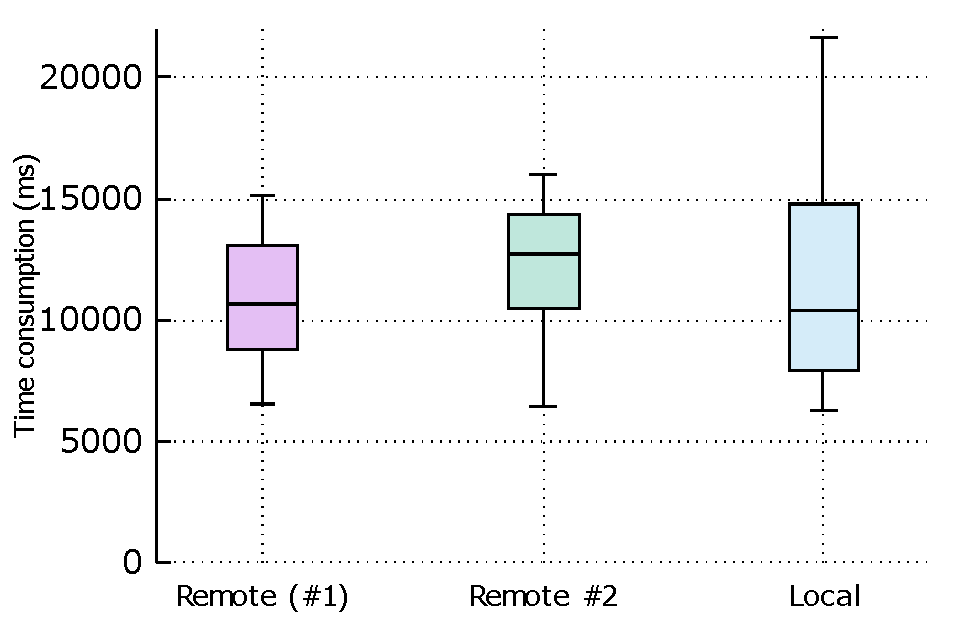
\includegraphics[width=.39\textwidth]{data/gps_perf.pdf}
		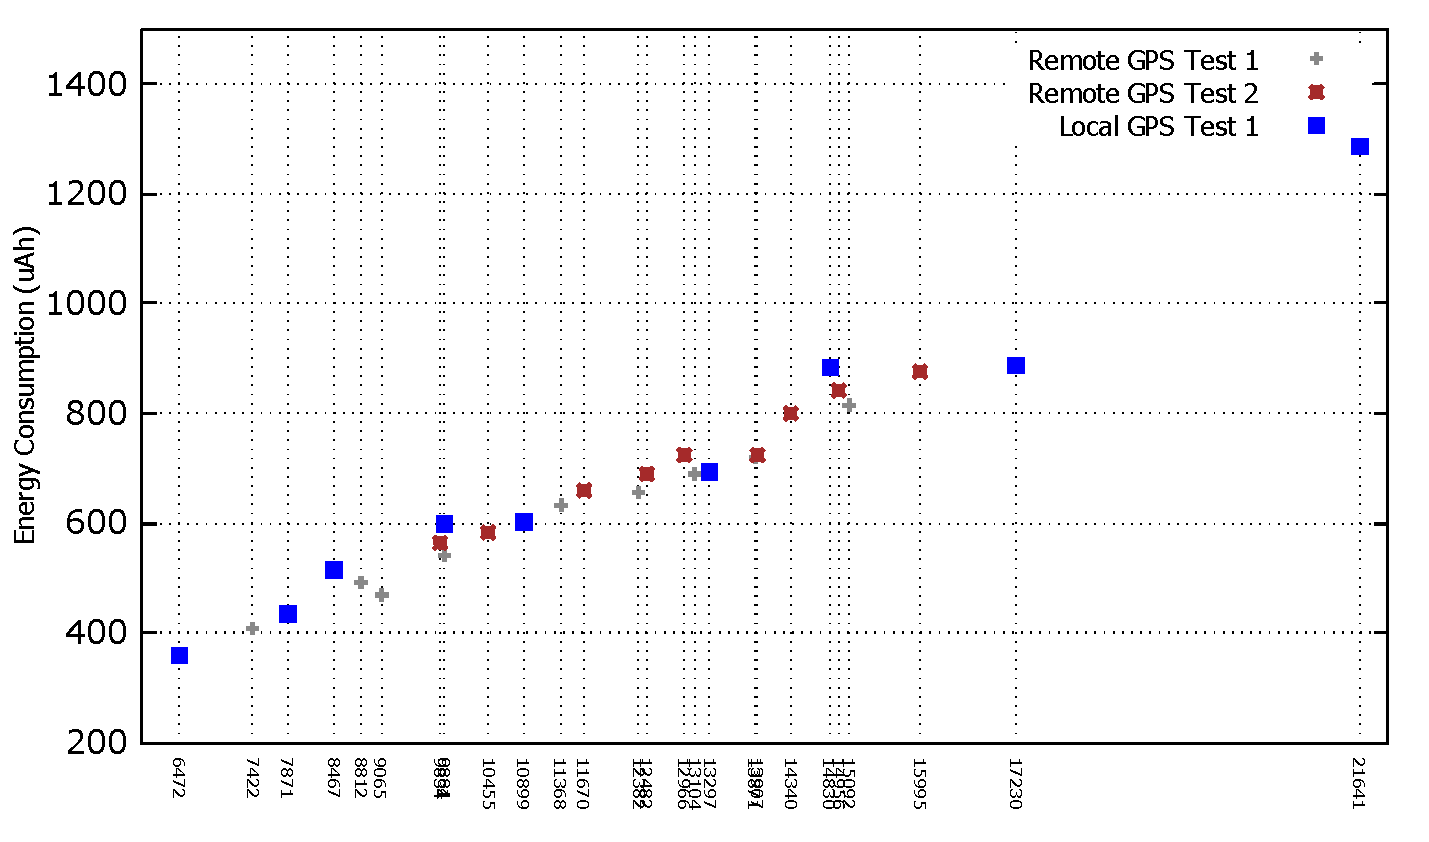
\includegraphics[width=.45\textwidth]{data/gps_energy_full.pdf}
	%}
	\caption{Performance and energy consumption comparison for GPS between remote and local executions}
	\label{fig:gps_perf}
\end{figure*}

Extracted from the above tests, the Figure \ref{fig:gps_total_energy} describes the distribution of energy consumptions among the 3 case tests. 

%\begin{figure}
	%\hspace*{0cm}
	%\resizebox{0.5\textwidth}{!}{
		%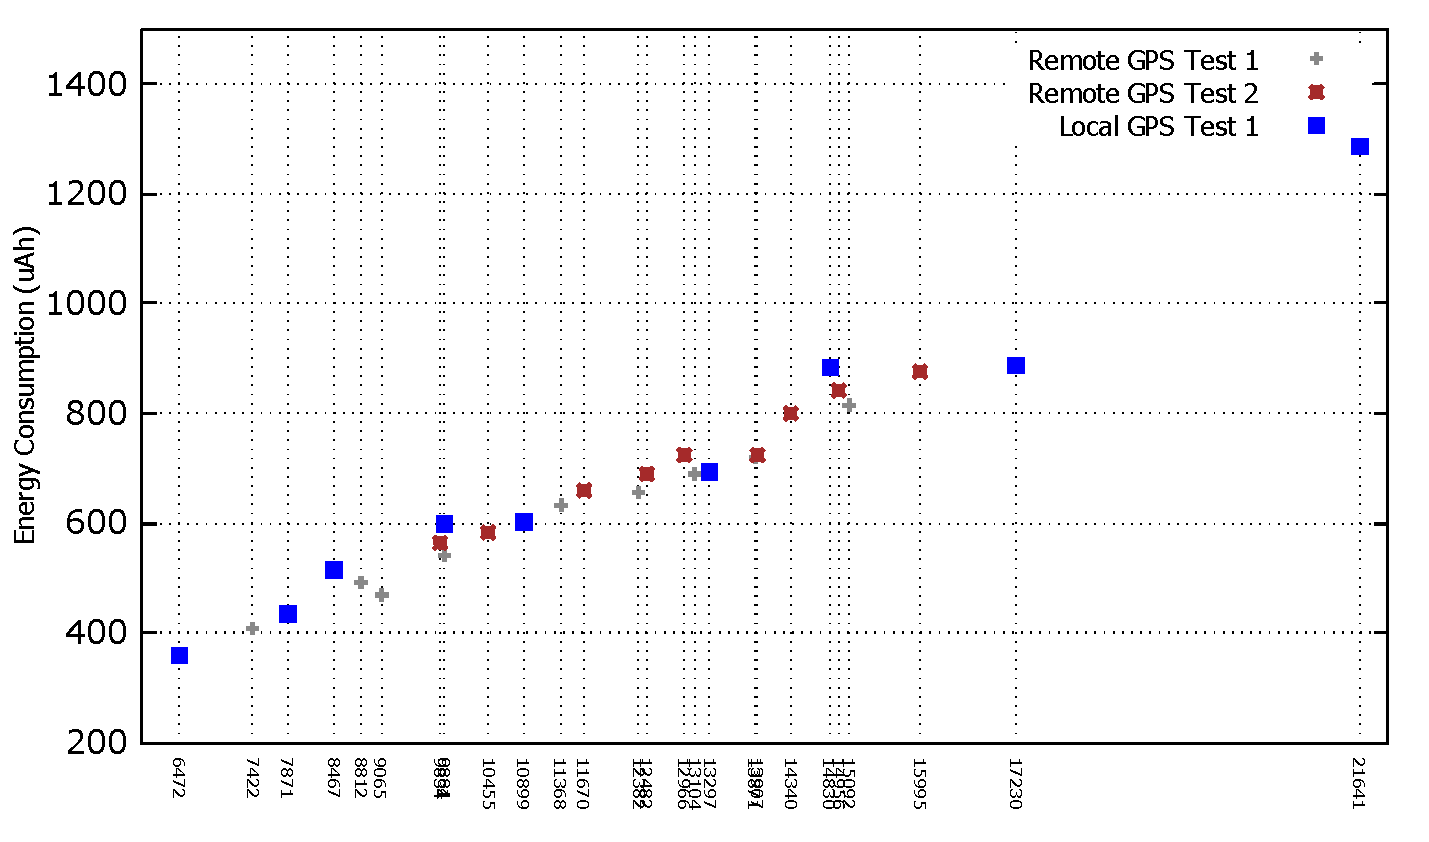
\includegraphics{data/gps_energy_full.pdf}
	%}
	%\caption{Energy consumption of GPS Share between remote and local executions}
	%\label{fig:gps_total_energy}
%\end{figure}

By applying interpolation to find trend lines for these energy distributions, we got $y = 0.0528388 \times x + 7.31948$ formula for test 1, $y = 0.0547221 \times x + 7.42138$ for test 2 and $y = 0.0575331 \times x - 12.9403$ for test 3. The trend line 3 has the biggest slope, or at the same amount of time it consumed more energy than the first two cases. As we might see, the difference between the slopes of line 3 and line 1, 2 are very slim, however due to our later tests on the weak caller (low battery), the difference will highly increase. 

\paragraph{Applications}
By integrating our system with either RetroSkeleton \cite{retro-skel} or Rio \cite{rio}, we can provide remote or local GPS location data without having to modify the current installed applications. Those systems provide interference methods to capture requests for system resources and instead inject their customized responses. 

\section{Related Work}
\label{sec:related}
These days, there are several similar approaches facilitating peer-to-peer wireless connection and multiple devices collaboration. 

Alljoyn Framework \cite{alljoyn} is an open source software framework making transparent of complexity of discover and communication to the developers. Providing interoperability functionality without any transport layer, Alljoyn make it easy to integrate and initiate. However since they tried to address multiple platforms: Android, iOS, Linux, Windows and even the other lightweight real-time operating systems, their package became huge and APIs is complicated to use. 

Before the Wi-Fi Direct available in software industry, many efforts to address P2P networks, Frank H. P. Fitzek et al. \cite{m_p2p_tutor} summarized the relevant papers focusing on this topic to demonstrate the initiative steps to establish the point-to-point collaborative Wi-Fi networks. Liam McNamara et al. published \cite{media_share} media sharing based on historical colocation information over urban transport using blue-tooth or any available wireless connections.

Since the modern mobile devices (phones and tablets) are featured with multiple network capabilities, many researches relied on these features to exchange resources and computations. Ardalan et al. designed Rio \cite{rio} bases on I/O device files to share contents and resources among the applications in different devices without having to modify them. Their use-cases addressed multi-system photography and gaming, singular SIM card for multi-devices, music and video sharing. Nairan Zhang et al. developed GameOn \cite{gameon} to utilize Wi-Fi P2P to establish non-Internet connection between the gamers, which majorly focuses on closed range network like in public transportation, bus or train. The other content sharing systems CAMEO \cite{cameo}, Spartacus \cite{spartacus} and GigaSight \cite{crowd-sourcing} try to detect closed range networks base on specific methods to distributed data. Utilizing Doppler effect applying on built-in microphones and speakers, Spartacus help can initiate and interact with nearby devices through pointing gesture with accuracy up to 90\% within distance of 3 meters.

In terms of improving energy consumption, offloading-featured systems like MAUI \cite{maui}, COMET \cite{comet}, \cite{cloud-offload}, \cite{mobile-cloud-middleware} or \cite{fuzzy-engine} address the heavy computations by offloading source code or execution module to server following multiple constraints and policies to release workload and energy consumed at client which is either mobile device or low computation capacity computer. 

\section{Future Work and Conclusions}
\label{sec:conc}
Our future research direction will 

In this paper, we have presented XXXXX, an extended distribution framework for resource-constraint mobile devices. 

%\section*{Acknowledgment}
%This research is supported by Utah State University through the RC Grant.

\balance
\bibliographystyle{abbrv}
\bibliography{references}

\end{document}

